\documentclass{article}
\usepackage{graphicx}
\usepackage{amsmath}
\usepackage{caption}
\usepackage{placeins}
\usepackage{amssymb}
\usepackage{amsfonts}
\usepackage{mathtools}
\usepackage{hyperref} 
\usepackage{listings}
\usepackage{xcolor}


\lstset{language=Python, 
        basicstyle=\ttfamily,
        keywordstyle=\color{blue}\bfseries,
        commentstyle=\color{green},
        stringstyle=\color{red},
        showstringspaces=false}

\begin{document}

\title{Homework Set 1, CPSC 8420-843}
\author{Matthew Collins}
\date{\today}
\maketitle

\section{Lasso}

The plots in Figure 1 compare the behavior of the Lasso regression coefficients as the regularization parameter $\lambda$ increases from $0.01$ to $1000$ using two different approaches: coordinate descent and Scikit-learn’s Lasso solver. Both methods display the expected behavior of Lasso regression, where the coefficients shrink towards zero as $\lambda$ increases, enforcing sparsity in the solution.

In the coordinate descent plot (left), the values of $x$ change significantly for small values of $\lambda$. As $\lambda$ increases, most coefficients are gradually driven to zero, with only a few remaining non-zero. This trend aligns with the behavior expected from Lasso regression, where larger $\lambda$ values penalize larger coefficients more heavily, ultimately reducing their magnitude. 

The Scikit-learn Lasso plot (right) demonstrates a similar pattern. Coefficients that start with larger magnitudes shrink towards zero as $\lambda$ increases. The overall behavior is consistent with that observed in the coordinate descent method: at low $\lambda$, coefficients vary more widely, while at higher $\lambda$ values, most coefficients become zero or very close to zero. 

Both methods exhibit very similar trends, particularly with respect to how coefficients are sparsified. The small discrepancies are due to the underlying differences in the optimization process used by the Scikit-learn solver and the coordinate descent implementation. However, the overall consistency between the two methods suggests that the coordinate descent implementation is functioning correctly.

\begin{figure}[htbp]
    \centering
    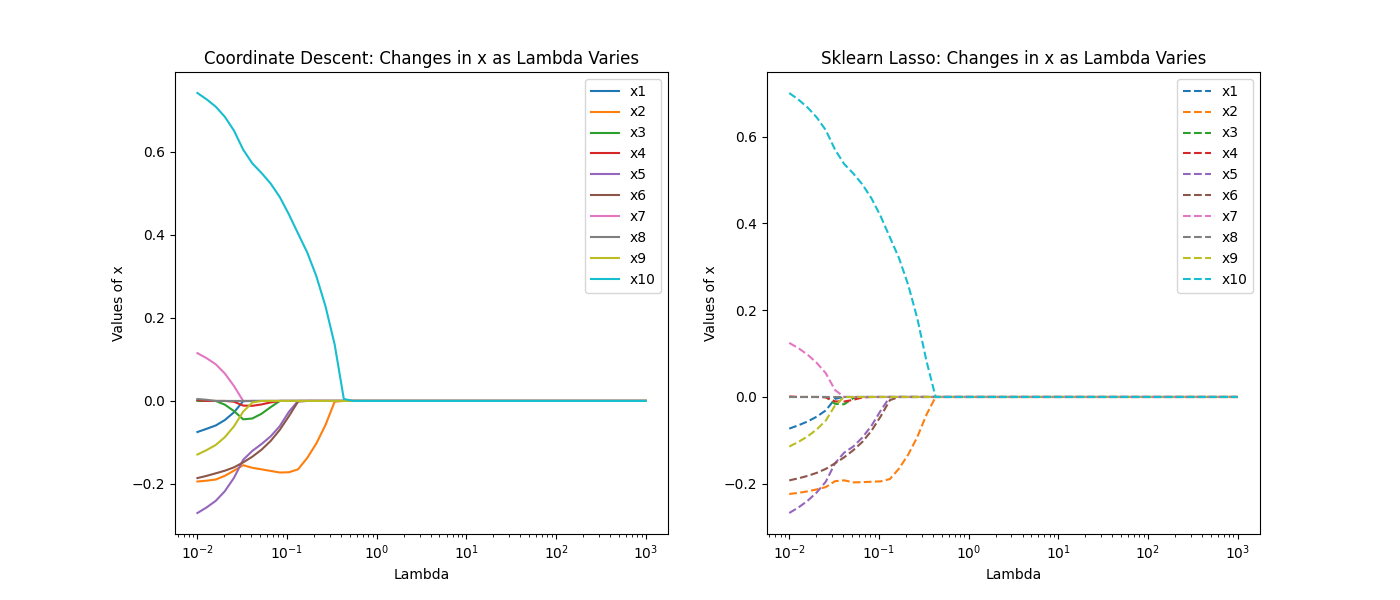
\includegraphics[width=\textwidth]{sln_figures/fig1.png}
    \caption{Comparison of changes in $x$ as $\lambda$ varies using Coordinate Descent (left) and Scikit-learn Lasso (right).}
\end{figure}
\FloatBarrier


\section{Least Squares Extension}


Let \( A \in \mathbb{R}^{n \times n} \), \( C \in \mathbb{R}^{n \times n} \), \( X \in \mathbb{R}^{n \times n} \), and \( Y \in \mathbb{R}^{n \times n} \) be matrices. The goal is to find \( X \) such that:

\[
A X + X C = Y
\]

The vectorization of a matrix product can be written as:

\[
\text{vec}(A X) = (I_n \otimes A) \text{vec}(X)
\]
\[
\text{vec}(X C) = (C^T \otimes I_n) \text{vec}(X)
\]

Thus, the original equation becomes:

\[
\text{vec}(A X + X C) = (I_n \otimes A) \text{vec}(X) + (C^T \otimes I_n) \text{vec}(X) = \text{vec}(Y)
\]

Simplifying this gives:

\[
(A \otimes I_n + I_n \otimes C^T) \text{vec}(X) = \text{vec}(Y)
\]

Let \( A_{\text{least\_squares}} = A \otimes I_n + I_n \otimes C^T \) and \( b = \text{vec}(Y) \). We now have the linear system:

\[
A_{\text{least\_squares}} \text{vec}(X) = b
\]

To solve for \( X \), we perform the singular value decomposition (SVD) of \( A_{\text{least\_squares}} \):

\[
A_{\text{least\_squares}} = U \Sigma V^T
\]

where \( U \) and \( V \) are orthogonal matrices, and \( \Sigma \) is a diagonal matrix containing the singular values of \( A_{\text{least\_squares}} \). The pseudoinverse of \( A_{\text{least\_squares}} \) is given by:

\[
A_{\text{least\_squares}}^+ = V \Sigma^+ U^T
\]

where \( \Sigma^+ \) contains the reciprocals of the non-zero singular values of \( A_{\text{least\_squares}} \).

Thus, the least squares solution is:

\[
\text{vec}(X) = A_{\text{least\_squares}}^+ b = V \Sigma^+ U^T b
\]

Finally, we reshape \( \text{vec}(X) \) back into an \( n \times n \) matrix to obtain the solution \( X \).



\begin{figure}[htbp]
    \centering
    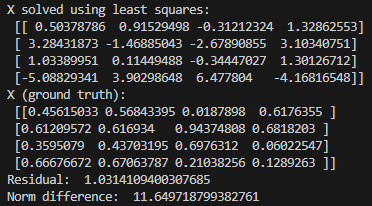
\includegraphics[width=\textwidth]{sln_figures/fig2.png}
    \caption{$X_{\text{least\_squares}}$, $X_{\text{ground\_truth}}$, Residual, and Norm Difference}
\end{figure}
\FloatBarrier

The results of the least squares solution in Figure 2 for the matrix equation \( A X + X C = Y \) provide insight into the performance of the algorithm. The residual, which measures the discrepancy between the left-hand side and the right-hand side of the equation, was approximately \( 1.03 \). This indicates that the computed solution, \( X_{\text{solution}} \), is fairly close to satisfying the equation. Given that the problem was solved using a least squares approach, a nonzero residual is expected. 

On the other hand, the norm difference between the computed solution \( X_{\text{solution}} \) and the ground truth \( X^* \) was found to be significantly larger, at approximately \( 11.65 \). This large difference indicates that while the computed solution satisfies the equation well (as reflected by the small residual), it is quite different from the true solution. The system may be underdetermined, meaning that multiple solutions exist that satisfy the equation. In such cases, the least squares approach may find a solution that minimizes the residual, but this solution may differ significantly from the ground truth. Addition of some kind of optimization algorithm such as gradient descent could possibly used to minimize the norm difference.

\section{Ridge Regression}


\[
\hat{\beta}(\lambda) = (A^T A + \lambda I)^{-1} A^T y
\]
The term \( (A^T A + \lambda I)^{-1} \) is the inverse of the regularized covariance matrix \( A^T A \), where \( \lambda I \) is a diagonal matrix scaled by \( \lambda \). As \( \lambda \) increases, the diagonal elements of \( A^T A + \lambda I \) increase, causing the overall inverse \( (A^T A + \lambda I)^{-1} \) to decrease in magnitude. This happens because larger values of \( \lambda \) make the matrix more "dominant" and reduce the influence of \( A^T A \).

Thus, as \( \lambda \) increases, the product \( (A^T A + \lambda I)^{-1} A^T y \) becomes smaller, resulting in a smaller norm \( \| \hat{\beta}(\lambda) \|_2 \).

\[
\| \hat{\beta}(\lambda_2) \|_2 \leq \| \hat{\beta}(\lambda_1) \|_2 \quad \text{for} \quad \lambda_1 < \lambda_2
\]

This directly shows that the norm of the ridge regression solution is a monotone decreasing function with respect to \( \lambda \).

\begin{figure}[htbp]
    \centering
    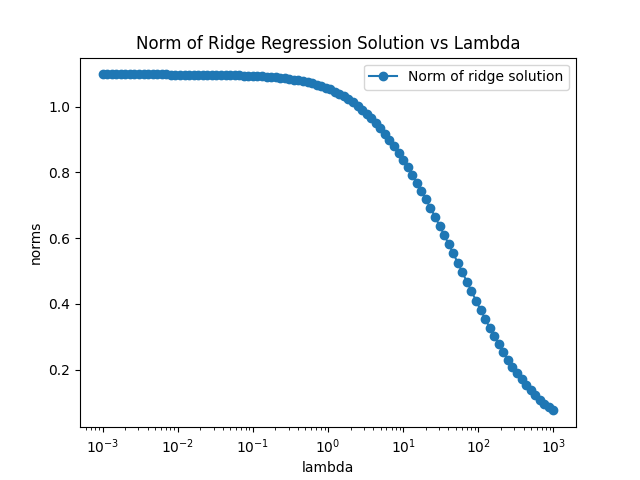
\includegraphics[width=\textwidth]{sln_figures/fig3.png}
    \caption{Norm of Ridge Regression as $\lambda$ Increases}
\end{figure}
\FloatBarrier


\section{Linear Regression and its Extension}

\subsection{Part One}
The Matlab code was converted to Python code, and the data was split into a training set and a testing set and shuffled~\ref{appendix:4.1}.


\subsection{Part Two}
In this assignment, the goal was to implement Ordinary Least Squares (OLS) regression on a dataset and compare the performance of this method with the built-in linear regression model from the Scikit-Learn library. I used a housing dataset, which was shuffled using a random permutation before splitting it into different training sizes of \( n = \{25, 50, 75, 100, 150, 200, 300\} \). For each of these training sizes, the training set was standardized using the Z-score normalization method from the SciPy library.

I computed the Mean Squared Error (MSE) on both the training set and the remaining data used as a test set. This was done for both the OLS implementation and the Scikit-Learn linear regression model. The OLS method was implemented by calculating the pseudo-inverse of the design matrix and then computing the weights (or regression coefficients) by multiplying this pseudo-inverse with the training labels \ref{appendix:4.2} 

The MSE for each training size was plotted for both methods, as shown in Figure~\ref{fig:mse_vs_tn}. The red line with diamond markers represents the MSE of the training set using the OLS method, and the black line with diamond markers shows the MSE on the test set for the OLS method. Similarly, the blue and yellow dotted lines represent the training and test MSE for the Scikit-Learn model, respectively.

We observe that the results from both the self-built Ordinary Least Squares (OLS) method and the Scikit-Learn linear regression model coincide for both the training and test data, validating the correctness of the custom OLS implementation. As more training data is included, the Mean Squared Error (MSE) for the training set increases slightly. This is because the model is exposed to more varied data, making it harder to perfectly fit all the training points, especially if the data contains noise or non-linearity. This leads to a slight increase in training error, which indicates reduced overfitting as the model generalizes better to unseen data. However, this increase in training MSE is gradual and reflects the model's improved generalization.

At the same time, as the model is trained on more data, its predictions on the test set become more accurate, resulting in a decrease in test MSE. This happens because the model learns a more accurate representation of the underlying data distribution, improving its ability to generalize to unseen data. Importantly, the test set size remains constant throughout the process, and the reduction in test MSE is due to better generalization, not a change in the size of the test set.

Eventually, the training and test error curves converge. This occurs because the training error increases slightly with more data while the test error decreases, leading to a balance between the model's performance on the training and test sets. When the curves meet, it indicates that the model has learned enough from the data to generalize well and no longer overfits the training set or underfits the test set.

\begin{figure}[h!]
    \centering
    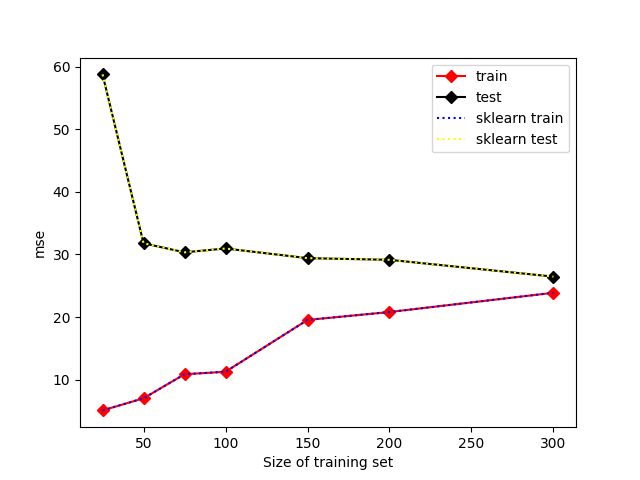
\includegraphics[width=0.7\textwidth]{sln_figures/fig4_2.png}
    \caption{Mean Squared Error vs. Training Set Size for OLS and Scikit-Learn Linear Regression}
    \label{fig:mse_vs_tn}
\end{figure}
\FloatBarrier


\subsection{Part Three}
In this assignment, the task was to expand the original features of the housing dataset to higher-order terms and evaluate how increasing the degree of polynomial expansion impacts the performance of the model. Specifically, the expansion involved replacing the original features with higher powers of the features (i.e., quadratic, cubic, and so on, up to degree 6). Interaction terms between features were ignored, meaning only pure polynomial terms were included in the expansion. The expanded features were standardized in the same way as the original features, and the expanded data set was treated consistently with the previously processed data.

It is important to note that due to certain binary features in the dataset (such as a feature that takes values 0 or 1), the degree expansion of those features results in the same values as the original set. This causes the design matrix to become non-invertible, meaning that the matrix \( A^T A \) cannot be inverted directly. To address this, the pseudoinverse function `\texttt{pinv()}` was used instead of the regular inverse `\texttt{inv()}` to ensure numerical stability and handle the non-invertibility of the matrix.

The custom function \texttt{ordinary\_least\_squares} was implemented to perform the least squares regression, using the pseudoinverse for the inversion step, while the Scikit-Learn \texttt{LinearRegression} function was also used for comparison. The Mean Squared Error (MSE) for both the training and test sets was calculated for each degree of expansion, and the results were plotted. The plot in Figure~\ref{fig:mse_vs_degree} shows the relationship between the MSE and the degree of feature expansion. The red line with diamond markers represents the training MSE for the custom Ordinary Least Squares (OLS) implementation, while the black line with diamond markers shows the test MSE for the OLS method. The blue and yellow dotted lines represent the training and test MSE for the Scikit-Learn linear regression model, respectively.

As shown in the plot, the test error initially decreases at degree 2, indicating that this level of feature expansion offers the best prediction in terms of minimizing the test set MSE. However, as the degree of polynomial expansion continues to increase, the test error rises sharply, indicating the onset of overfitting. This overfitting is further evidenced by the fact that the training error remains low, even as more complex features are added. The model becomes increasingly complex with higher degrees, which allows it to fit the training data almost perfectly, but at the cost of poor generalization to unseen test data. This behavior illustrates the trade-off between bias and variance as model complexity increases. The sharp increase in test MSE at higher degrees, particularly at degrees 5 and 6, highlights this overfitting problem.

The results of the custom function were cross-validated using the Scikit-Learn package, and the trends observed in the self-built function matched those obtained using Scikit-Learn, further validating the implementation.


\begin{figure}[h!]
    \centering
    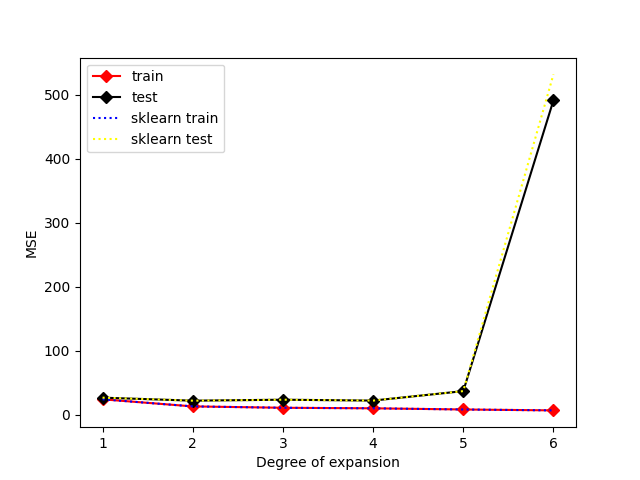
\includegraphics[width=0.7\textwidth]{sln_figures/fig4_3.png}
    \caption{MSE for training and test data as a function of the degree of polynomial expansion}
    \label{fig:mse_vs_degree}
\end{figure}

\FloatBarrier



\subsection{Part Four}

In this assignment, the goal was to apply ridge regression to a degree 6 polynomial expansion of the housing dataset features. The ridge regression adds an $L_2$ regularization term to the least squares cost function, which helps reduce overfitting by penalizing large coefficients. The regularization strength is controlled by the parameter $\lambda$, and in this assignment, we explored the effect of different values of $\lambda$ on the model's performance.

We performed the degree 6 polynomial expansion by creating higher-order terms for each feature in the dataset. This was done by raising the original features to the powers of 2 through 6, then concatenating these expanded features with the original ones. The expanded feature matrix was then standardized using Z-score normalization to ensure that all features were on the same scale.

The ridge regression was performed using both a custom function, \texttt{ridge\_least\_squares}, which computes the pseudoinverse of the design matrix and incorporates the regularization term, and the \texttt{Ridge} function from Scikit-Learn. For comparison, we computed the Mean Squared Error (MSE) for both the training and test sets as a function of $\lambda$, where $\lambda$ was varied over a log scale between $10^{-10}$ and $10^{10}$.

The results are presented in Figure~\ref{fig:ridge_plot}. The green line with diamond markers represents the training MSE for the custom ridge regression, while the cyan line shows the test MSE for the custom implementation. Similarly, the blue and red lines represent the training and test MSE for the Scikit-Learn \texttt{Ridge} model.

As observed in the plot, the test MSE initially decreases as $\lambda$ increases, indicating that a small amount of regularization improves the model's generalization by reducing overfitting. However, as $\lambda$ continues to increase, the test error begins to rise again. This occurs because higher values of $\lambda$ excessively penalize the model coefficients, leading to underfitting, where the model is too constrained to capture the complexity of the data. The training MSE, on the other hand, increases steadily with increasing $\lambda$, as larger regularization forces the model to fit the training data less closely.

Overall, the behavior of ridge regression demonstrates the trade-off between bias and variance: small $\lambda$ values lead to overfitting (low bias but high variance), while large $\lambda$ values lead to underfitting (high bias but low variance).

\begin{figure}[h!]
    \centering
    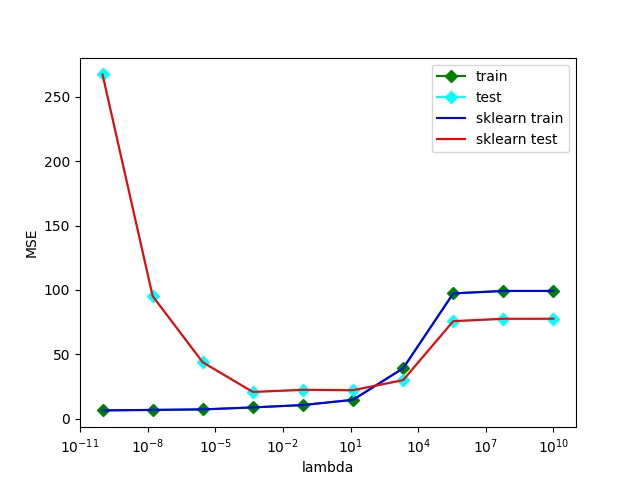
\includegraphics[width=0.8\textwidth]{sln_figures/fig4_4.png}
    \caption{MSE vs. $\lambda$ for the training and test sets with ridge regression.}
    \label{fig:ridge_plot}
\end{figure}

\FloatBarrier



When $\lambda$ is very small in ridge regression, the solution closely resembles that of conventional ordinary least squares (OLS) regression. Therefore, with a small $\lambda$, we observe a significant gap between the training and test MSE, especially in high-degree polynomial expansions like the 6-degree expansion shown in Figure~\ref{fig:ridge_plot}. This gap arises because the model overfits the training data, resulting in low training error but high test error due to poor generalization.

The ridge regression implementation in the self-built function was cross-validated using the Scikit-Learn \texttt{Ridge} function, as shown in the plot. The pseudo-inverse was used to ensure numerical stability in solving the regression, especially because high-degree polynomial expansions often lead to ill-conditioned design matrices. Ridge regression also includes a bias (or intercept) term, which was not regularized, ensuring that only the coefficients of the features were penalized. This is done by multiplying the $\lambda$ regularization term with a $(p \times p)$ identity matrix, leaving the intercept term unregularized.

As $\lambda$ increases, the model is regularized more strongly, which reduces the variance and prevents overfitting. This leads to a decrease in the test MSE. However, as $\lambda$ becomes too large, some important coefficients are shrunk too much, causing the model to underfit, and the bias increases. This results in a rise in both the training and test MSE at higher values of $\lambda$. In summary, ridge regression balances bias and variance: small $\lambda$ values can lead to overfitting, while large $\lambda$ values can cause underfitting.



\begin{thebibliography}{99}

\bibitem{chan1} Chan, Stanley H. *Introduction to Probability for Data Science*. Michigan Publishing, 2023, pp. 449-457.

\bibitem{lasso_impl} Xavier Bourret Sicotte. Lasso Implementation. Available at: \url{https://xavierbourretsicotte.github.io/lasso_implementation.html}.

\bibitem{regularized_linreg} Towards Data Science. Regularized Linear Regression Models. Available at: \url{https://towardsdatascience.com/regularized-linear-regression-models-dcf5aa662ab9}.

\bibitem{linear_to_ridge} Towards Data Science. From Linear Regression to Ridge Regression. Available at: \url{https://towardsdatascience.com/from-linear-regression-to-ridge-regression-the-lasso-and-the-elastic-net-4eaecaf5f7e6}.

\bibitem{chan2} Chan, Stanley H. *Introduction to Probability for Data Science*. Michigan Publishing, 2023, pp. 396-422.

\bibitem{stackexchange} Math Stack Exchange. Least Squares Solution to Underdetermined Lyapunov Equation. Available at: \url{https://math.stackexchange.com/questions/4808422/least-squares-solution-to-underdetermined-lyapunov-equation}.

\bibitem{aimspress} AIMS Press. Solving Underdetermined Linear Systems. Available at: \url{https://www.aimspress.com/article/doi/10.3934/mmc.2021009?viewType=HTML}.

\bibitem{chan3} Chan, Stanley H. *Introduction to Probability for Data Science*. Michigan Publishing, 2023, pp. 440-448.

\bibitem{ridge_regression} Medium. Ridge Regression Step-by-Step Introduction. Available at: \url{https://medium.com/@msoczi/ridge-regression-step-by-step-introduction-with-example-0d22dddb7d54}.

\bibitem{chan4} Chan, Stanley H. *Introduction to Probability for Data Science*. Michigan Publishing, 2023, Chapter 7.

\bibitem{ols_medium1} Medium. Understanding Ordinary Least Squares (OLS) and Its Applications in Machine Learning. Available at: \url{https://medium.com/@dahami/understanding-ordinary-least-squares-ols-and-its-applications-in-statistics-machine-learning-ad2c13681501}.

\bibitem{linear_regression_scikit1} Mashkar Haris. Linear Regression in Python Using Scikit-Learn. Available at: \url{https://mashkarharis.medium.com/linear-regression-in-python-scikit-learn-526b57a11a09}.

\bibitem{contactsunny} ContactSunny. Linear Regression in Python Using Scikit-Learn. Available at: \url{https://contactsunny.medium.com/linear-regression-in-python-using-scikit-learn-f0f7b125a204}.

\bibitem{ridge_regression_mastering} Medium. Mastering Ridge Regression. Available at: \url{https://medium.com/@bernardolago/mastering-ridge-regression-a-key-to-taming-data-complexity-98b67d343087}.

\bibitem{ridge_lasso_practical} Medium. Ridge and Lasso Regression: Practical Implementation in Python. Available at: \url{https://alok05.medium.com/ridge-and-lasso-regression-practical-implementation-in-python-c4a813a99bce}.

\end{thebibliography}







\appendix
\section{Appendix}



\subsection{Lasso}\label{appendix:1}
\lstinputlisting[language=Python]{hw1_1_lasso.py}


\subsection{Least Square Extension}\label{appendix:2}
\lstinputlisting[language=Python]{hw1_2_lse.py}


\subsection{Ridge Regression Monotone}\label{appendix:3}
\lstinputlisting[language=Python]{hw1_3_ridge.py}

\subsection{Loading Dataset}\label{appendix:4.1}
\lstinputlisting[language=Python]{hw1_4_housing.py}

\subsection{MSE vs Training Size}\label{appendix:4.2}
\lstinputlisting[language=Python]{hw1_4_2_housing.py}

\subsection{MSE vs Degree}\label{appendix:4.3}
\lstinputlisting[language=Python]{hw1_4_3_housing.py}

\subsection{Ridge Regression}\label{appendix:4.4}
\lstinputlisting[language=Python]{hw1_4_4_housing.py}



\end{document}



